\label{sec:forward_model}
The modelling framework developed here builds on the work by \cite{wheeler2017fragmentcloud,wheeler2018atmospheric} and extends it in several ways. The specific theoretical model by \cite{wheeler2017fragmentcloud} was chosen since it is the most general, meaning that it can be specialized to behave like most of the other models in the literature with a specific set of parameters.
In this work, the set of coordinates and equations is adjusted such that the model tracks the meteoroid and its fragments in three dimensional space and calculates the locations of impacts on the surface.

\subsection{Initial descent phase}

The position of the meteoroid is described with coordinates $(x, y, z)$ defined as follows: $z$ is the height above sea level, $x$ is the downrange distance measured from the start of the simulation, and $y$ is the distance of the meteoroid from its original projected straight path. Note that in this work both $x$ and $y$ are projected onto the planetary surface. The direction of the velocity vector is described by two angles ($\theta$ and $\phi$). $\phi$ is the trajectory angle in the $xy$ plane, and $\theta$ is the trajectory angle w.r.t. the $xy$ plane. A horizontal trajectory has an angle $\theta = 0$, and we define $\theta = \frac{\pi}{2}$ to indicate that the velocity vector points straight downward along the $z$ axis.

For these coordinates, the standard meteoroid physics equations \citep[e.g.][]{passey1980effects} for a planet of radius $R_p$ are
\begin{align}
    \label{eq:dvdt} \frac{dv}{dt} &= -\frac{C_D \rho_a v^2 \pi r^2}{2m} + g\sin(\theta) \\
    \frac{dm}{dt} &= -\frac{C_\mathrm{ab}}{2}\rho_a v^3 \pi r^2 \\
    \frac{d\theta}{dt} &= \frac{g\cos(\theta)}{v} - \frac{C_L \rho_a \pi r^2 v}{2m} - \frac{v\cos(\theta)}{R_p + z} \\
    \frac{dz}{dt} &= -v\sin(\theta) \\
    \frac{dx}{dt} &= v\cos(\theta)\cos(\phi)\frac{R_p}{R_p + z} \\
    \label{eq:dydt} \frac{dy}{dt} &= v\cos(\theta)\sin(\phi)\frac{R_p}{R_p + z} \\
    \frac{d\phi}{dt} &= 0\,,
\end{align}
where $C_D$, $C_\mathrm{ab}$ and $C_L$ are the coefficients of drag, ablation and lift respectively, $\rho_a$ is the air density, and $g$ is the gravitational acceleration, which is a function of $z$. The introduction of the angle $\phi$ and two coordinates for downrange distance, $x$ and $y$, allows the calculation of impact locations on the two-dimensional planetary surface. The differential equations for $x$ and $y$ are derived in Appendix~\ref{sec:meteoroid_eq_deriv}.

For the differential equation of $r$, there are two possibilities. First, we may simply assume that before breakup, $r$ is constant. Since the mass $m$ will still be changing due to ablation, the implicit assumption is that the meteoroid will deform into an ellipsoid, flying in a configuration of maximum drag. On the other hand, \cite{avramenko2014simulation} suggested calculating $\frac{dr}{dt}$ in a way that keeps the shape of the meteoroid spherical:
\begin{equation}
    \frac{dr}{dt} = \frac{1}{3}\frac{r}{m}\frac{dm}{dt}\,.
    \label{eq:CRM_1}
\end{equation}
Note that this is a slightly different but equivalent form compared to what is presented in the paper, cf. Appendix~\ref{sec:CRM_details}.

\subsection{Breakup}

We assume that a meteoroid fragments when its aerodynamic strength $\sigma$ is exceeded by the difference in air pressure between opposing sides. The biggest pressure differential will be between the leading edge and trailing edge. The pressure at the leading edge, behind the bow shock, is called the stagnation pressure. The pressure on the other end, in the meteoroid wake, is nearly zero \citep{passey1980effects}. Therefore break up will occur when
\begin{equation}
    \rho_a v^2 = \sigma\,,
\end{equation}
where $\rho_a$ is the air pressure, and $v$ is the meteoroid velocity.

At this point, there are two established ways to model the breakup process, both of which are implemented in our library.
The first one was established by \cite{passey1980effects}, and was subsequently used and expanded upon by Artemieva et al., for example in their works \citep{artemieva1996interaction,artemieva2001motion}. We refer to it here as the separate fragments (SF) model. As the name suggests, in this model the meteoroid breaks up into a number of pieces that are subsequently modeled individually and may break up themselves further on in the simulation.

The second approach describes the breakup process as a continuous deformation of a single object. This is meant to describe the shape and other properties of an expanding cloud of small fragments. There are several versions of this approach, which have been referred to as pancake-type models \citep{wheeler2017fragmentcloud}. 

Most recently, \cite{wheeler2017fragmentcloud} proposed a hybrid model that combines the previous two approaches, which they call a ``fragment-cloud'' model.

\subsubsection{Separate fragments model}
\label{sec:fragments_model}
In this model, the breakup process is approximated by splitting the meteoroid into several distinct fragments, which subsequently may or may not get separated enough to form independent bow shocks \citep{artemieva1996interaction}. In this work we assume that fragments always separate enough to form distinct bow shocks. For a meteoroid splitting into two fragments, \cite{passey1980effects} argue that the interaction between the bow shocks will accelerate both fragments away from each other perpendicular to the current trajectory. When the separation is large enough that the bow shocks are completely separate, the fragments will have a relative velocity of
\begin{equation}
    V_T = V_i\sqrt{\frac{3}{2}C\frac{R_b}{R_f}\frac{\rho_a}{\rho_f}}\,,
    \label{eq:v_t}
\end{equation}
where $C$ is a dimensionless factor, $R_b$ is the radius of the larger fragment, $R_f$ radius of the smaller fragment, $\rho_a$ is the air density, $\rho_f$ is the density of the smaller fragment,
and $V_i$ is the velocity of the meteoroid just before fragmentation. $C$ indicates the distance $d = C\cdot R_b$ at which the interaction between the two bow shocks stops. \cite{artemieva2001motion} calculate that $\frac{3}{2}C\approx 0.19$ for two cylindrically shaped fragments of the same size and weight. This falls towards the lower end of the range of $[0.02, 1.52]$ initially proposed \citep{passey1980effects}.

At this point, several sources of randomness are introduced into the model. The first one cannot be avoided: $V_T$ from Eq.~\ref{eq:v_t} is a vector in the plane perpendicular to the meteoroid trajectory just before break up occurs. This still leaves one degree of freedom, the orientation of $V_T$ on this plane; cf. Appendix~\ref{sec:frag_detail} for full details.

The second potential source of randomness is the number and relative mass of fragments generated in the breakup process. As in \cite{wheeler2018atmospheric}, the number of new fragments per break up event is regarded as a fixed input parameter in the library. However, the model developed here allows the simulation to randomly choose the relative masses of fragments over a predefined range of possible values, as proposed by \cite{newland2019CFM18}. 

With these first two choices, all properties of the generated fragments are determined except for the aerodynamic strength. The canonical argument is that the break up will occur along the weakest part of the meteoroid. With these weak parts breaking up, the remaining fragments should have a greater strength than the larger meteoroid before break up. This is typically captured by the following Weibull-like scaling equation \citep{weibull1951statistical,artemieva2001motion}:
\begin{equation}
    \sigma_f = \sigma_b \left(\frac{m_b}{m_f}\right)^\alpha\,,
    \label{eq:weibull}
\end{equation}
which increases the strength with decreasing fragment size. $\sigma_f, m_f$ and $\sigma_b, m_b$ are the strength and mass of the fragment and meteoroid respectively, and $\alpha$ is a positive scaling parameter.
\cite{artemieva2001motion} suggested to introduce a factor of randomness into this scaling relation as well. We have therefore implemented an option to multiply $\sigma_f$ from Eq.~\ref{eq:weibull} by a factor randomly chosen according to
\begin{equation*}
    \sigma_f = \sigma_b \left(\frac{m_b}{m_f}\right)^\alpha 10^x\,,\quad x \sim \mathcal{N}(0, \delta)\,,
\end{equation*}
where the standard deviation $\delta$ is a fixed input parameter.

\subsubsection{Pancake-type models}
\label{sec:cloud_model}
The library offers the following three models of this type. They all describe the meteoroid fragments as an expanding cloud of debris. The cloud as a whole still follows the same laws of atmospheric descent and ablation outlined in the standard meteoroid physics equations. The description of how the the cloud radius increases differs between models. The first one was introduced by \cite{hills1993fragmentation}. As long as the aerodynamic pressure $\rho_a v^2$ at the leading edge exceeds the aerodynamic strength of the initial meteoroid, the cloud radius increases as follows:
\begin{equation}
    \frac{dr}{dt} = v\sqrt{\frac{7}{2}\alpha\frac{\rho_a}{\rho_m}}\,,
    \label{eq:DCM}
\end{equation}
where $\rho_m$ is the density of the meteoroid material, and $\alpha$ is a dimensionless constant. \cite{hills1993fragmentation} found $\alpha \sim 1$ to be in good agreement with their data, while in a more recent study, \cite{wheeler2018atmospheric} found $\alpha \approx 0.6$ to be a better fit in their case. 

The second model was proposed by \cite{chyba1993tunguska} in which the second derivative of $r$ is defined as
\begin{equation}
    \frac{d^2r}{dr^2} = \frac{C_D \rho_a v^2}{2r\rho_m}\,,
    \label{eq:PM}
\end{equation}
$C_D$ is a drag coefficient of order unity. The third model supported by the library was presented in a study of the Chelyabinsk fireball by \cite{avramenko2014simulation}. According to their model, while the ram pressure exceeds the aerodynamic strength $\sigma$, the radius of the cloud expands with rate
\begin{equation}
    \frac{dr}{dt} = \frac{1}{3}\frac{r}{m} \frac{dm}{dt} +  C_\mathrm{fr} \frac{r}{2} \frac{\sqrt{\rho_a v^2 - \sigma}}{m^{1/3}\rho_m^{1/6}}\,,
    \label{eq:CRM}
\end{equation}
where $C_\mathrm{fr}$ is a dimensionless factor that they found to be of order $C_\mathrm{fr} \sim 1.5$.

In all three variations, the debris cloud experiences rapid deceleration due to aerodynamic drag. At some point, the ram pressure drops below the strength of the original meteoroid again. \cite{hills1998damage} assume that the debris cloud then stops expanding and that the debris particles continue descending under a common bow shock. In our library, we therefore continue the simulation with $\frac{dr}{dt} = 0$.

\subsubsection{Fragment-cloud model}
\label{sec:fragment_cloud_model}
The idea for this hybrid model was first presented at a conference \citep{mehta2015break} and later studied by \cite{wheeler2017fragmentcloud}.
The model is conceptually very similar to the separate fragments approach.
The key difference is that as a result of each break up event, in addition to breaking up into a small number of fragments, a portion of the meteoroid mass forms a debris cloud that is described with a pancake-type model.

\cite{wheeler2018atmospheric} expanded the fragment-cloud model by introducing an inner structure to the meteoroid, illustrated in figure~\ref{fig:FCMv2}. This changes how the initial break up works. Instead of treating the meteoroid as a homogeneous object, the meteoroid is modeled to break up into predefined groups of fragments, each with potentially different density, size and strength. This allows modeling of very inhomogeneous meteoroids, so-called rubble piles. It also allows the meteoroid to break up into smaller weak parts and larger strong parts, which is not possible in the separate fragments model that defines the strength with a Weibull scaling law. \cite{wheeler2018atmospheric} achieved good agreement with terrestrial light-curve data when they assumed such a structure.

\begin{figure*}
    \centering
    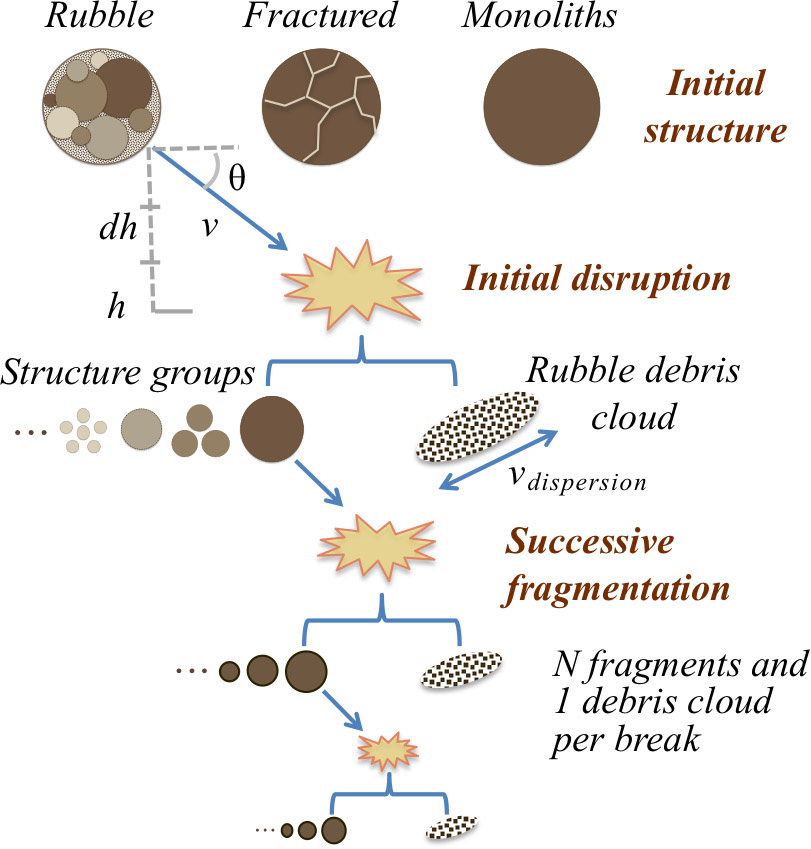
\includegraphics[width=0.7\textwidth]{figures/wheeler_diagram.jpg}
    \caption{FCM model diagram, taken from \cite{wheeler2018atmospheric}.
        A meteoroid is modeled to enter a planetary atmosphere with a speed $v$ and a trajectory angle $\theta$ relative to the ground. When the ram pressure exceeds its aerodynamic strength at height $h$ above the ground, it fragments into different structural groups, and a debris cloud. The debris cloud is described with a ``pancake''-style model. The fragments descend further into the atmosphere and may undergo successive fragmentation when their aerodynamic strength is exceeded.\label{fig:FCMv2}}
\end{figure*}

\subsection{Impact}

Once fragments of the meteoroid impact the ground, we use a well-established scaling relationship to determine the crater diameters $D$ \citep{holsapple1987scaling}.
\begin{align}
    \pi_2 &= \frac{g_0 r}{v_z^2}\,,\quad\pi_3 = \frac{Y}{\rho_t v_z^2}\,,\quad\pi_4 = \frac{\rho_t}{\rho_i}\,, \nonumber \\
    e_1 &= \frac{6\nu - 2 - \mu}{3\mu}\,,\quad e_2 = \frac{6\nu-2}{3\mu} \,, \nonumber \\
    e_3 &= \frac{2+\mu}{2}\,,\quad e_4 = -\frac{3\mu}{2 + \mu} \nonumber \\
    \pi_v &= K_1 \left[\pi_2 \pi_4^{e_1} + K_2 \left(\pi_3 \pi_4^{e_2}\right)^{e_3}\right]^{e_4} \nonumber \\
    V &= \pi_v \frac{m}{\rho_t} \nonumber \\
    D &= 2f_\mathrm{rim} K_r V^{1/3} \label{eq:holsapple2}
\end{align}
This relationship cover a large range of potential surface properties and impact scenarios.
$g_0$ is the gravitational acceleration at the impact location, $r$ the radius of the impacting fragment, $v_z$ its vertical velocity, $m$ its mass and $\rho_i$ its density. Without the factor $f_\mathrm{rim}$, these laws calculate the crater diameter at pre-impact surface level.
Some of the crater ejecta typically form a rim around the crater, which is what is visible on satellite images. We therefore multiply the result by $f_\mathrm{rim} \sim 1.3$ to match observations more closely \citep{daubar2020newcrater}. The ground is modeled with the following properties: Density $\rho_t$, strength $Y$, and a number of coefficients $K_1$, $K_2$, $K_r$, $\mu$, $\nu$. While the library allows for arbitrary values to be set, this work used parameters appropriate for a weak granular soil \citep{holsapple1987scaling}, listed in table~\ref{tab:holsapple_coeff}.  

In cases where two or more craters overlap, they are combined into a single crater with a volume equal to the sum of the two crater volumes.

\begin{table}[htbp]
    \centering
    \begin{tabular}{c|c}
        $\rho_t$ & $1.5\,\mathrm{\frac{g}{cm^3}}$ \\
        $Y$ & $50\,\mathrm{kPa}$ \\
        $K_1$ & 0.133 \\
        $K_2$ & 1.0 \\
        $K_r$ & 1.25 \\
        $\mu$ & 0.41 \\
        $\nu$ & 0.40 \\
        $f_\mathrm{rim}$ & 1.3
    \end{tabular}
    \caption{Coefficients used for Holsapple scaling laws (eq.~\ref{eq:holsapple2}).}
    \label{tab:holsapple_coeff}
\end{table}

\subsection{Implementation}
\label{sec:implementation}
The main goal of the implementation was to develop a flexible, high-performance library. The implementation used in a similar work \citep{newland2019CFM18} was available, but was severely limited in performance and scalability. Its main limiting factor was that it was written entirely in Python. It performed well enough to be usable for entirely cloud-driven models, as well as for scenarios with few fragments. However, for meteoroids heavier than a few kilograms, the number of fragments produced by the model can soon reach tens of thousands, which brings the solver to a crawl. Because of the iterative nature of any ODE solver, the solver loop cannot be vectorised.
We therefore re-implemented the forward model in a compiled language, C++.
For ease of use, we developed a Python API for it, and plan to release the entire library as a Python package.

The library provides multiple ODE solver options for equations \ref{eq:dvdt} - \ref{eq:dydt} and \ref{eq:DCM} - \ref{eq:CRM}.
Contrary to what \cite{wheeler2017fragmentcloud} proposed, our implementation uses a more conventional time stepping scheme, rather than setting a fixed height step size of e.g. $\delta z = 10\unit{m}$.

\subsubsection{Performance optimizations}
The library provides the option to use either a fixed or an adaptive time step size that adjusts to the estimated local error of each fragment and debris cloud individually. It offers second and fourth order accurate schemes. In our convergence analysis, we found that with a variable step size, our model achieves the same accuracy at $1/3$ of the number of iterations compared to a fixed time step size. It avoids wasting computation time early on in the simulation, when not much is happening in the thin upper atmosphere, while significantly decreasing the step size when fragmentation is happening and rapidly ablating/decelerating debris clouds and tiny fragments are formed.

Opting for a time stepping scheme instead of Wheeler et al.'s fixed $z$ step poses two challenges that we had to address. First, any time stepping scheme will overshoot the moment of impact ($z_\mathrm{final} < z_\mathrm{ground}$), which is not the case if the $z$ step size is chosen correctly. The solution is straightforward: we decrease the last step size such that $z_\mathrm{final} = z_\mathrm{ground}$ exactly. Second, in the case of a variable step size, which is different for each fragment in the simulation, calculating the energy deposition in the atmosphere per unit height, $dE/dz$, requires interpolation. As a side note, a similar overshooting problem and the solution that we came up with is described in appendix~\ref{sec:overshoot}. This last problem is also present in the ODE solving approach that \cite{wheeler2017fragmentcloud} used.

Another significant performance advantage of our model is that we exclude fragments from the simulation that are no longer relevant in two ways: First, if a fragment or a debris cloud would produce an impact crater that is smaller than a pre-defined threshold, and second if a debris cloud has deposited practically all its kinetic energy into the atmosphere. Both avoid needlessly tracking tiny fragments that would form craters too small to detect. 
All these techniques combined yield an enormous performance increase; we see between two and three orders of magnitude improvement compared to the Python implementation.
It is now feasible to run Monte-Carlo simulations within minutes instead of hours. Potential use cases of the library are numerous. We utilize it in the following sections to investigate martian crater clusters.
